\section{Înregistrarea unei cereri}

	Pentru a înregistra o cerere cât mai ușor și fără probleme, aplicația se împarte modular în mai multe categorii, observabile în figurile~\ref{fig:register_avariator}, ~\ref{fig:register_cerere_despagubire}, ~\ref{fig:register_deteriorat}, ~\ref{fig:register_poze}.

	Cea mai mare categorie și cea mai importantă este despre informațiile generale legate de cererea de despăgubire, ce se poate observa în figura~\ref{fig:register_informatii_generale}.

	\begin{figure}
		\centering
		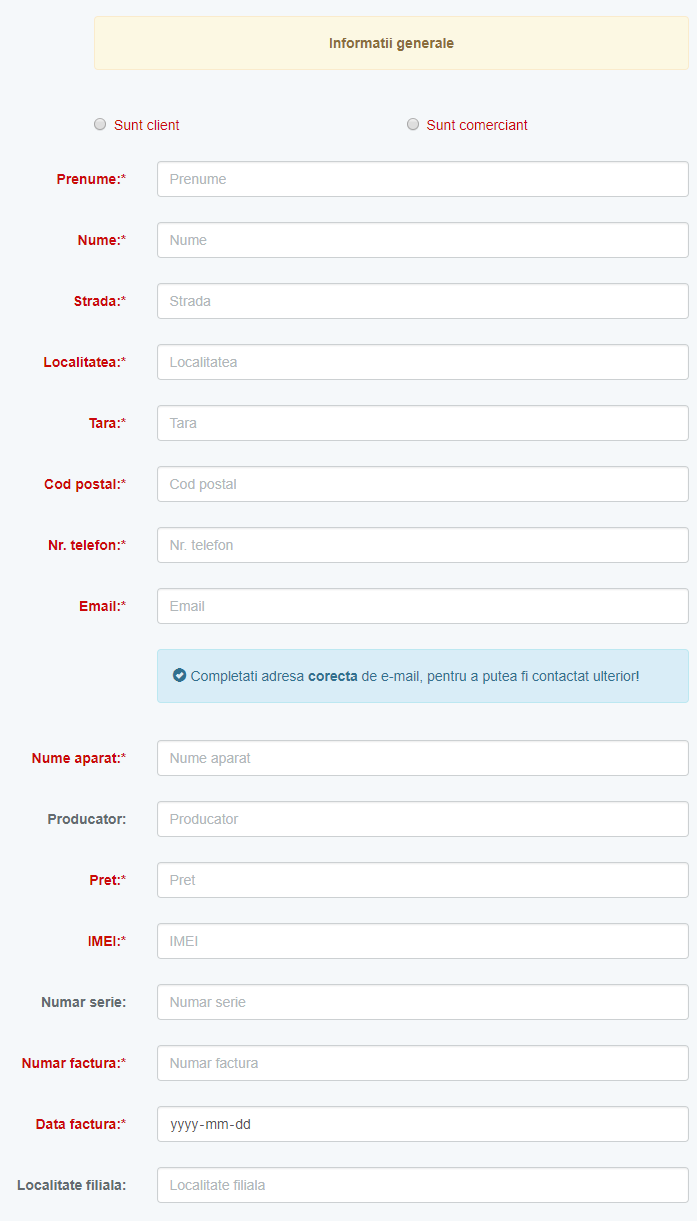
\includegraphics[width=0.8\linewidth]{../imagini/register_informatii_generale.png}
		\caption{Informații generale}
		\label{fig:register_informatii_generale}
	\end{figure}

	\begin{figure}
		\centering
		\subfigure[Informații despre cine a provocat avarierea produsului]{
			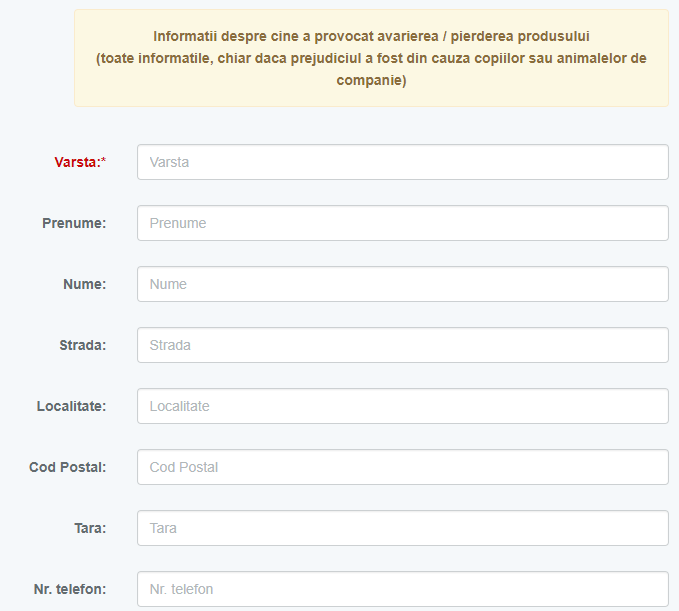
\includegraphics[width=0.4\linewidth]{../imagini/register_avariator.png}
			\label{fig:register_avariator}
		}
		\subfigure[Informații despre cererea de despăgubire]{
			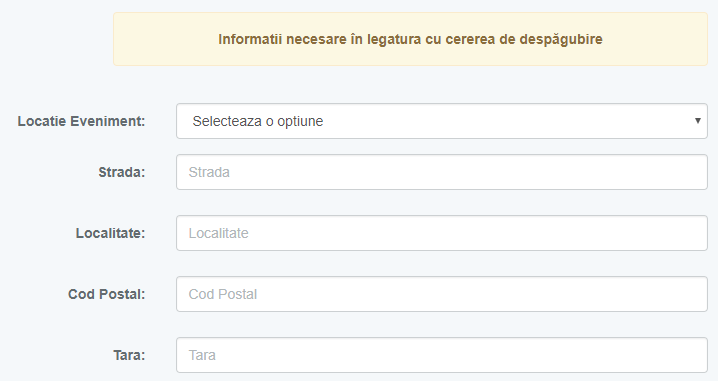
\includegraphics[width=0.4\linewidth]{../imagini/register_cerere_despagubire.png}
			\label{fig:register_cerere_despagubire}
		} \\
		\subfigure[Descrierea evenimentelor]{
			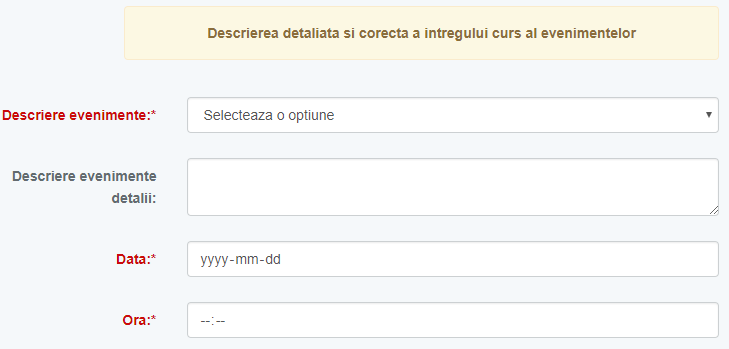
\includegraphics[width=0.4\linewidth]{../imagini/register_decurs.png}
			\label{fig:register_decurs}
		}
		\subfigure[Problemele dispozitivului]{
			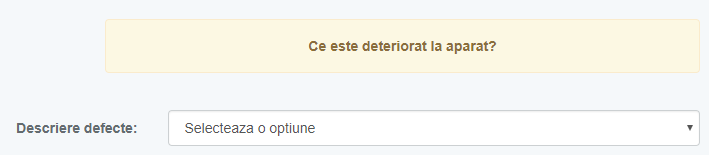
\includegraphics[width=0.4\linewidth]{../imagini/register_deteriorat.png}
			\label{fig:register_deteriorat}
		}
		\subfigure[Avertizare încărcare poze]{
		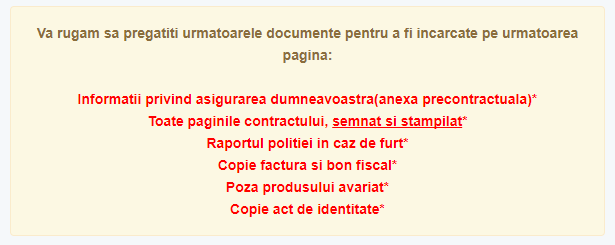
\includegraphics[width=\linewidth]{../imagini/register_poze.png}
			\label{fig:register_poze}
		}
		\caption{Câmpurile de completat în cererea de despăgubire}
	\end{figure}

	După ce vor fi completate câmpurile obligatorii, înainte de a se trimite cererea, clientul este avertizat cu un dialog:
	\begin{verbatim}
	Asigurați-vă că ați completat formularul corespuzător!
	Următoarea solicitare pentru cererea curentă poate fi
	înregistrată abia în următorul interval de 24 de ore.
	\end{verbatim}

	După ce se înregistrează cererea, se trimite un mail către client și utilizatorii sistemului, pentru a certifica crearea unei noi cereri de despăgubire cu toate datele completate.

	În figura~\ref{fig:message_new_claim} se poate observa structura mesajului.

	\begin{figure}
		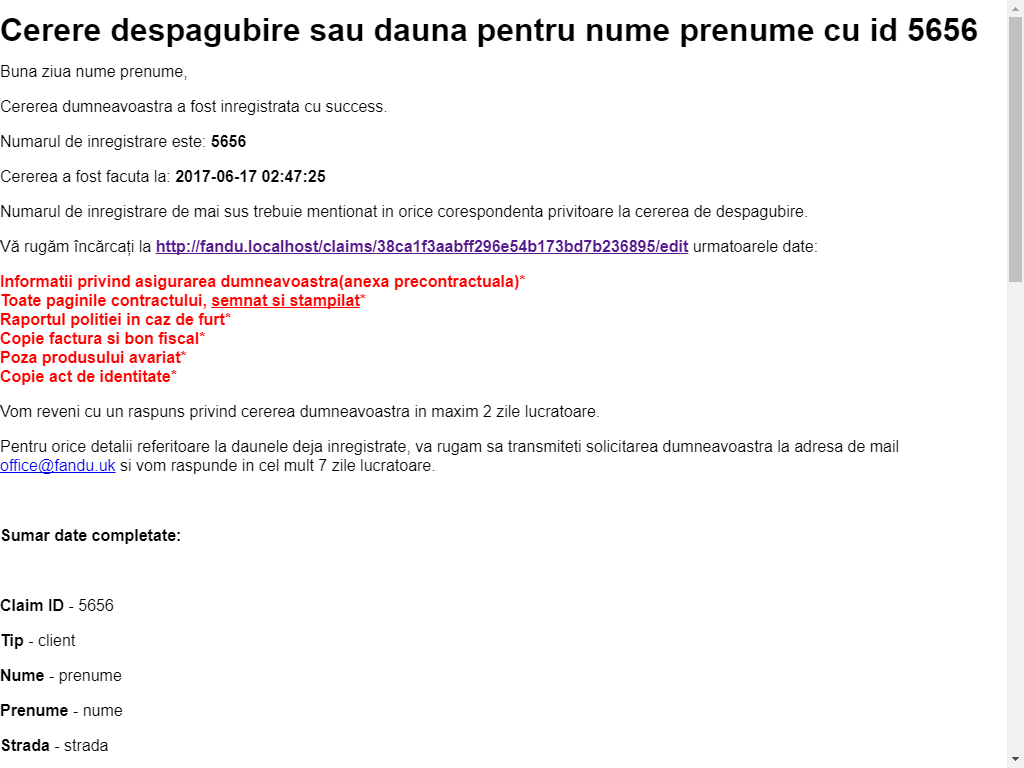
\includegraphics[width=\linewidth]{../imagini/message_new_claim.png}
		\caption{Mesajul trimis de sistem către client și utilizatorii sistemului}
		\label{fig:message_new_claim}
	\end{figure}

	În același timp, utilizatorul este redirecționat către pagina de încărcare poze, vizibilă în figura~\ref{fig:report_incarcare_poze}.

	\begin{figure}
		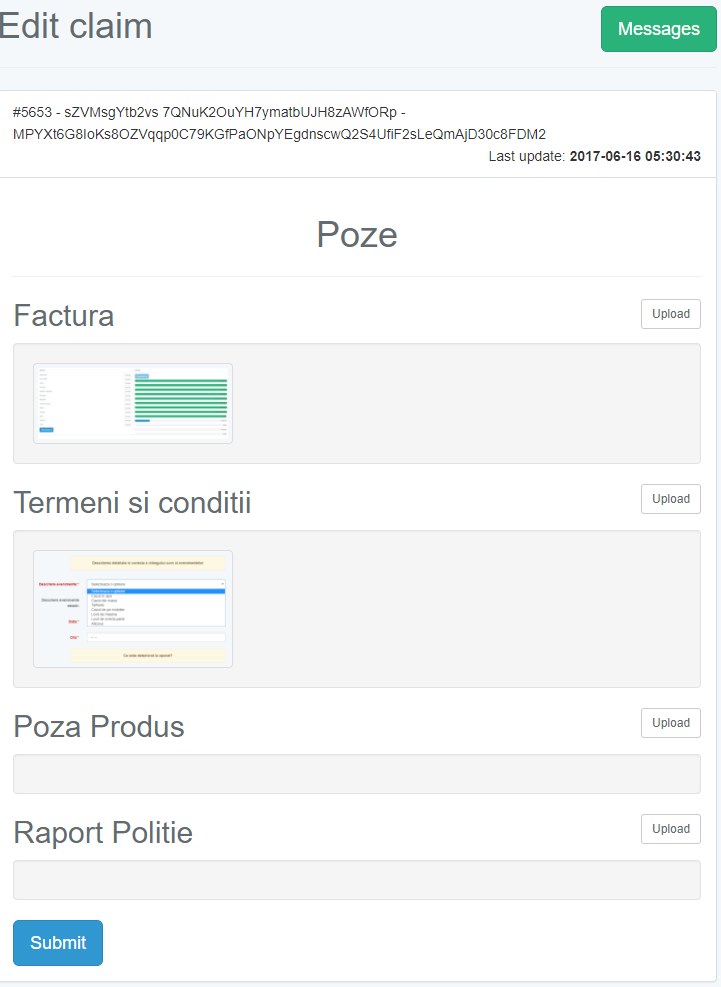
\includegraphics[width=\linewidth]{../imagini/report_incarcare_poze.png}
		\caption{Formularul de încărcare a pozelor}
		\label{fig:report_incarcare_poze}
	\end{figure}


